%
% $RCSfile: broken_type_system.tex,v $
%
% Copyright (c) 2004. Christian Heller. All rights reserved.
%
% No copying, altering, distribution or any other actions concerning this
% document, except after explicit permission by the author!
% At some later point in time, this document is planned to be put under
% the GNU FDL license. For now, _everything_ is _restricted_ by the author.
%
% http://www.cybop.net
% - Cybernetics Oriented Programming -
%
% http://www.resmedicinae.org
% - Information in Medicine -
%
% @author Christian Heller <christian.heller@tuxtax.de>
%

\subsection{Broken Type System}
\label{broken_type_system_heading}

Languages like \emph{Smalltalk} or the \emph{Common Lisp Object System} (CLOS)
offer reflective mechanisms \cite{buschmann}. The \emph{C++ Standard Library},
also known as \emph{libstdc++} \cite{libstdcpp}, has a \emph{type\_info} class
providing meta information that \emph{C++} innately does not have.

In the \emph{Java} framework \cite{java}, finally, the basic \emph{java.lang.*}
package contains the top-most super class \emph{java.lang.Object}. All other
classes in the framework inherit from it. Additionally, the package contains a
class \emph{java.lang.Class} which, among others, keeps reflective (meta) type
information about a \emph{Java} class':

\begin{itemize}
    \item[-] Package
    \item[-] Name
    \item[-] Superior Class
    \item[-] Interfaces
    \item[-] Fields
    \item[-] Methods
    \item[-] Constructors
    \item[-] Modifiers
    \item[-] Member Classes
\end{itemize}

\begin{figure}[ht]
    \begin{center}
        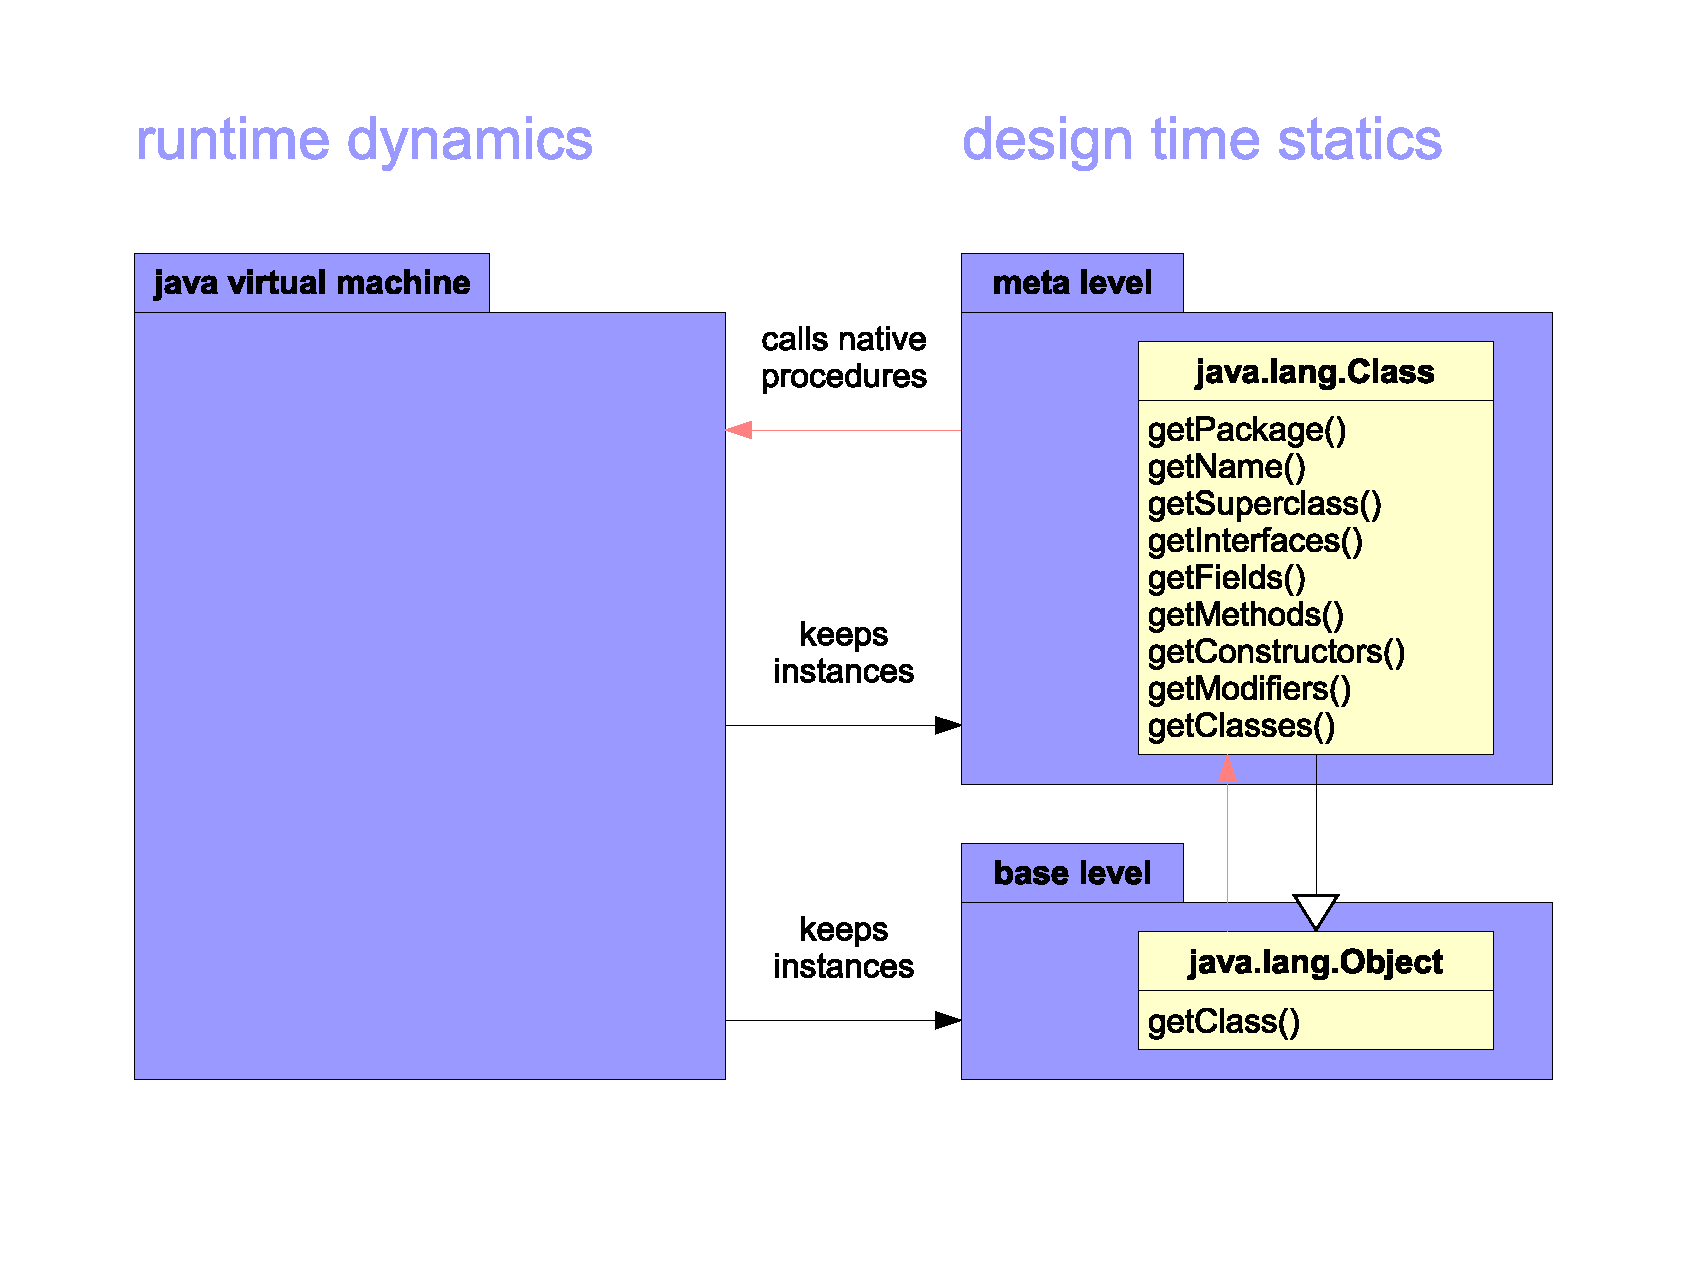
\includegraphics[scale=0.3]{vector/typesystem.eps}
        \caption{Java Type System}
        \label{typesystem_figure}
    \end{center}
\end{figure}

Via the \emph{getClass()} method which they inherit from \emph{java. lang.Object}
(figure \ref{typesystem_figure}), all Java classes have access to that reflective
information in their meta class. The meta class \emph{java.lang.Class} itself
uses so-called \emph{native} methods to access the information in the
\emph{Java Virtual Machine} (JVM).

The JVM operates on a level underneath the actual application, close to the
\emph{Operating System} (OS). It interprets the Java application source code and
resolves all object-oriented- into procedural structures, and finally low-level
system instructions. All runtime objects, that is class instances, are hold in
dynamic structures internal to the JVM. That is why \emph{native} methods need
to be used to access and change the runtime structure or behaviour of objects.

One problem that becomes obvious when inspecting figure \ref{typesystem_figure}
is the existence of a \emph{Bidirectional Dependency}, also called
\emph{Circular Reference}. The two sub dependencies causing it are:

\begin{enumerate}
    \item \emph{Inheritance} of \emph{java.lang.Class} from \emph{java.lang.Object}
        which is due to the rule that all Java classes need to inherit from the
        top-most framework class
    \item \emph{Association} from \emph{java.lang.Object} to \emph{java.lang.Class}
        which enables every object to access its meta class using the
        \emph{getClass()} method
\end{enumerate}

The avoidance of circular references is one of the most basic principles of
computer programming (section \ref{bidirectional_dependency_heading}). The
disadvantage of bidirectional dependencies between meta- and basic level is
also mentioned by Buschmann \cite{buschmann}. If meta classes in the kind of
\emph{java.lang.Class} define the structure and behaviour of all basic classes
inheriting from \emph{java.lang. Object}, then those meta classes in turn should
\emph{not} themselves inherit from \emph{java.lang.Object}.

Another problem is the mixed and redundant storage of meta information which
Jonathon Tidswell \cite{josgeneral} even calls a \emph{Broken Type System}. He
writes: \textit{A careful examination of the classes in the standard runtime will
show that they are not strictly instances of java.lang.Class (hint: statics).}
Gilbert Carl Herschberger II \cite{josgeneral} calls the separation of
reflection and wrappers an \emph{Inconsistent Design}. Java classes are based
on many different kinds of type information:

\begin{itemize}
    \item[-] Structure applied by the JVM through the usage of the \emph{class} keyword
    \item[-] Meta information supplied by the \emph{java.lang.Class} class
    \item[-] Reflective information provided by \emph{java.lang.reflect.*}
    \item[-] Wrapper classes for primitive types in \emph{java.lang.*}
    \item[-] Dynamically created array classes, without having an array class file
\end{itemize}

The fact that the \emph{java.lang.Class} class which is to provide meta
information \emph{about} classes is a \emph{Class} itself is an antagonism. It
is true that that meta class is made \emph{final} to avoid its extension by
inheriting subclasses. But correctly, it should not be a class at all.

Yet how can this paradoxon be resolved? Obviously, one of the two dependencies
between \emph{java.lang.Object} and \emph{java.lang.Class} needs to be cut. But
then either the \emph{java.lang. Object} class would not be able to access its meta
information anymore or the \emph{java.lang.Class} class would not be available as
runtime object to other polymorphic data structures. One solution could be to
merge both classes, so that each object, by default, has the necessary methods
to access its meta information. But as it turns out, this would not be a real
solution, just a \emph{Shift} of the problem to another level. As mentioned above,
the JVM keeps all instances (objects) in internal, dynamic structures. If objects
were allowed to access these internal structures via native methods (procedures),
a similar kind of bidirectional dependency, between the JVM and its stored objects,
would occur.

One finally has to ask whether the usage and manipulation of meta information is
really necessary at all! If objects did not have a \emph{static} structure
consisting of certain attributes and methods, as defined by the software
developer at design time, but instead based on a uniform, \emph{dynamically}
changeable structure -- the need to use reflective mechanisms might disappear.
More research has to be done on this topic.

There are other Java-related points to be criticised. Although it is worth
noting they exist, these are \emph{not} explained in detail here, since this
document wants to focus on general concepts. Gilbert Carl Herschberger II
\cite{josgeneral} mentions the problematic issue of \emph{Pre-Conditions},
leading to corresponding \emph{Assumptions}. After him, such work-arounds were
necessary to break circular references in Java:

\begin{itemize}
    \item[-] Each JVM must pre-define an \emph{Internal Meta Class}, implemented
        in machine code and \emph{not} available as Java bytecode in a class file.
        The \emph{java.lang.Class} as base meta class for all Java classes depends
        on that internal meta class and assumes its existance.
    \item[-] A JVM pre-defines one \emph{Primordial Class Loader}, implemented in
        machine code and resolved at compile-time. Since additional class loaders
        need to know their meta class when being created, they have to assume the
        primordial class loader exists so that, using it, their meta class can be
        created first.
\end{itemize}

Jonathon Tidswell \cite{josgeneral} is of the opinion that there are a number of
security issues related to the design of Java, for example:

\begin{itemize}
    \item[-] Global names not local references are used for security
    \item[-] Wrappers and names are used for reflection
\end{itemize}

Even though most of the issues raised in this section are rather Java-specific,
many of them apply to other programming languages as well. \emph{Smalltalk}
\cite{smalltalk} and \emph{CLU} \cite{clu}, for example, make primitive types
look like classes and do not need special \emph{Wrapper} classes like Java. But
when digging deep enough, one will find that this is \emph{Syntactic Sugar}, as
Peter J. Landin used to call additions to the syntax of a computer language
that do not affect its expressiveness but make it \emph{sweeter} for humans to
use \cite{wikipedia}.
